\documentclass[11pt,a4paper]{article}
\usepackage[margin=2.0cm]{geometry}
\usepackage[T1]{fontenc}
\usepackage{lmodern}
\usepackage{graphicx}
\usepackage{booktabs}
\usepackage{float}
\usepackage{caption}
\usepackage{enumitem}
\usepackage{amsmath}
\usepackage{xcolor}
\usepackage[hidelinks]{hyperref}
\usepackage{xurl}
\usepackage{titlesec}
\graphicspath{{figures/}}
\setlist{itemsep=2pt,topsep=3pt}
\captionsetup{font=small,labelfont=bf}
\titleformat{\section}[display]{\normalfont\Large\bfseries}{\normalsize Section \thesection}{2pt}{}
\titlespacing*{\section}{0pt}{14pt}{8pt}
\newif\ifsecbreak \secbreaktrue
\AddToHook{cmd/section/before}{\ifsecbreak\clearpage\fi}
\newcommand{\obs}{\paragraph{Observations}}
\newcommand{\settings}[1]{\noindent\textbf{Settings.} #1\par\medskip}

\begin{document}

% ---------------------------------------------------------------- title
\begin{titlepage}
\centering
\vspace*{3cm}
{\LARGE\bfseries Synthetic 12-Lead ECG Generation\\[4pt] for Imbalanced Rhythm Classification\par}
\vspace{0.8cm}
{\large From beat stitching to latent diffusion: generation, quality filtering,\\ augmentation and realism on PTB-XL\par}
\vspace{2.5cm}
{\large Submitted by\\[4pt] \textbf{Shivank Mishra}\\ 2024ADPS0823G\par}
\vspace{1.2cm}
{\large Code: \url{https://github.com/shivankmishra144droid/Quality-Aware-Synthetic-Data-Augmentation-for-ECG-Classification}\par}
\vfill
{\large November 2026\par}
\end{titlepage}

\tableofcontents
\clearpage

% ---------------------------------------------------------------- key findings
\section*{Key Findings}
\addcontentsline{toc}{section}{Key Findings}

\noindent\fbox{\parbox{\dimexpr\linewidth-2\fboxsep-2\fboxrule}{
\textbf{Final generator status.} Latent diffusion model \textbf{C-M}: autoencoder (12$\times$1000 $\rightarrow$
16$\times$125 latent) + S4 denoiser with 16 layers, width 128, state 64 (5.9\,M parameters), v-prediction,
classifier-free guidance 2, 50 DDIM steps. Trained for 100k steps on Google Colab and Kaggle GPUs.\\[3pt]
\textbf{Validation realism} (feature-judge AUC, 0.5 = indistinguishable from real):
C-M \textbf{0.796\,$\pm$\,0.016} vs beat stitching 0.965\,$\pm$\,0.005; pre-registered verdict \textbf{better}.
Across three further sampling runs C-M scores 0.795--0.818. No training ECG is copied.}}

\begin{itemize}
\item \textbf{Beat stitching works as a first generator.} Learned beat templates with a rule-based rhythm model carry
  most of the class information: a classifier trained only on synthetic ECGs reaches 0.678 balanced accuracy on
  real ECGs (0.873 when trained on real ECGs). Whole-ECG diffusion at 1.5\,M parameters did not produce a regular
  heartbeat (Section~\ref{sec:gen1}).
\item \textbf{The quality score ranks samples, but quality filtering does not beat random selection.} Top-scored
  synthetic ECGs give 0.743 train-on-synthetic balanced accuracy against 0.672 random and 0.582 bottom-scored.
  As augmentation, filtered and random selection are equivalent: $-0.0041$ macro-F1 over 40 runs (Section~\ref{sec:filter}).
\item \textbf{Synthetic augmentation raises untuned macro-F1, but the gain is a decision-threshold effect.} Random
  synthetic data beats real-only training (+0.036 test macro-F1, 40/40 runs). However, AUPRC does not change, and
  once per-class thresholds are tuned on validation, 70--85\,\% of the gap closes (Section~\ref{sec:threshold}).
\item \textbf{Synthetic ECGs are detected through their noise, not their beats.} A judge built on 25 standard ECG
  features separates beat-stitched ECGs from real ones (AUC 0.973). The giveaways are residual noise statistics, beat-to-beat
  similarity and baseline wander. QRS width and amplitudes are realistic (Section~\ref{sec:realism}).
\item \textbf{Latent diffusion overtakes beat stitching once it is scaled up.} The autoencoder sets a realism
  ceiling of 0.627. A small latent model (0.8\,M) improves with training time (dev 0.967 $\rightarrow$ 0.922).
  The 5.9\,M model C-M reaches 0.796 on validation. Rhythm conditioning by R-peak maps controls heart rate in the
  medians but reduces realism (Sections~\ref{sec:latent}--\ref{sec:scale}).
\end{itemize}

\clearpage
\secbreakfalse
\listoffigures
\listoftables
\secbreaktrue
\clearpage

% ---------------------------------------------------------------- 1
\section{Introduction}
Rhythm classifiers trained on PTB-XL see far fewer minority-rhythm ECGs than sinus rhythm ones: SR is about 85\,\% of
the four-class data. Synthetic ECGs are a common remedy. This project asks three connected questions:
\begin{enumerate}
\item Can a generator trained on PTB-XL produce class-faithful 10-second, 12-lead ECGs on a 4\,GB laptop GPU?
\item Does selecting the \emph{best} synthetic ECGs (quality filtering) help more than selecting random ones, and does
  synthetic augmentation help at all once it is evaluated carefully?
\item What makes synthetic ECGs detectable, and can a learned whole-ECG model become more realistic than a
  hand-built pipeline?
\end{enumerate}
The work was done as a series of studies, each with its decisions written down before the main run (pre-registered).
Studies 1--3 used the test split for their registered analyses. The latent diffusion work (Sections~\ref{sec:latent}
and~\ref{sec:scale}) uses only the training and validation splits.

% ---------------------------------------------------------------- 2
\section{Data and Setup}
\subsection{Data}
PTB-XL v1.0.1 at 100\,Hz (10\,s, 12 leads). A recording is kept if exactly one of the rhythm labels SR, AFIB, STACH
or SBRAD is present: 19,759 recordings from 17,320 patients. The split is a patient-level 70/15/15 split (seed 42)
with no patient overlap: train SR 11,741 / AFIB 1,056 / STACH 568 / SBRAD 446; validation 2,960; test 2,988. Each
lead is z-scored with training-split statistics only. For the latent diffusion work, the training split is divided by
patient into a \emph{fit} part (11,719 ECGs) and a \emph{dev} part (2,092 ECGs). All tuning is done on dev.

\subsection{Baseline classifier}
A CNN-LSTM (46,756 parameters): two Conv1d blocks with batch norm, ReLU and max-pooling, then an LSTM(64), dropout
0.3 and a linear layer. It is trained with Adam (learning rate $10^{-3}$, weight decay $10^{-4}$, batch 64) and
class-weighted cross-entropy $w_c = n/(4n_c)$.

\begin{table}[H]\centering\small
\begin{tabular}{lccccc}\toprule
 & SR & AFIB & STACH & SBRAD & macro \\\midrule
test F1 & 0.955 & 0.877 & 0.805 & \textbf{0.497} & 0.783 \\
test recall & 0.926 & 0.897 & 0.917 & 0.779 & 0.880 \\\bottomrule
\end{tabular}
\caption{Real-only baseline. SBRAD is the weakest class: 122 true-SR test ECGs are predicted SBRAD.}
\end{table}

\subsection{Metrics and notation}
\begin{table}[H]\centering\small
\begin{tabular}{p{3.4cm}p{11.2cm}}\toprule
Term & Meaning \\\midrule
TSTR & Train on synthetic, test on real: the baseline trained on 440 synthetic ECGs per class only, scored on real
       validation ECGs (balanced accuracy). \\
untuned / tuned F1 & Macro-F1 with argmax decisions / with per-class log-probability offsets fitted on validation. \\
AUPRC & Area under the precision--recall curve. It does not depend on the decision threshold. \\
feature judge & Gradient-boosted classifier on 25 clinical ECG features (heart-rate variability, QRS width,
       amplitudes, noise statistics), trained to separate real from synthetic ECGs. AUC over five patient-grouped
       splits (mean $\pm$ SD); 0.5 = indistinguishable. \\
floor / ceiling & Judge AUC of real vs real (two patient halves) / of real vs autoencoder reconstructions. \\
HR-W & Wasserstein distance between real and synthetic heart-rate distributions (bpm). \\
coverage & Fraction of real ECGs with a synthetic neighbour in a task embedding (diversity). \\
membership AUC & Whether training ECGs lie closer to synthetic ones than unseen ECGs do (0.5 = no copying). \\\bottomrule
\end{tabular}
\caption{Metrics and notation used in the tables.}
\end{table}

% ---------------------------------------------------------------- 3
\section{Generator 1: Beat Stitching}\label{sec:gen1}
\settings{Rhythm comes from a statistical model, and only beat morphology is learned.
(1)~\emph{Templates}: for each training ECG, the median beat in a fixed window from R$-$250\,ms to R$+$450\,ms
(8 independent leads), giving 13,244 clean templates.
(2)~\emph{Template generator}: a class-conditional, v-prediction SSSD diffusion model (8 layers $\times$ 64) trained
on the templates.
(3)~\emph{Assembly}: per-class RR series from a fitted distribution of mean RR and RR variability (AR(1) for sinus
classes, gamma-distributed RR for AFIB). Templates are placed by overlap-add with respiratory modulation. Residual
noise and baseline wander are added as Gaussian processes with the real cross-lead spectrum, and the four limb leads
are derived.}

\begin{figure}[H]\centering
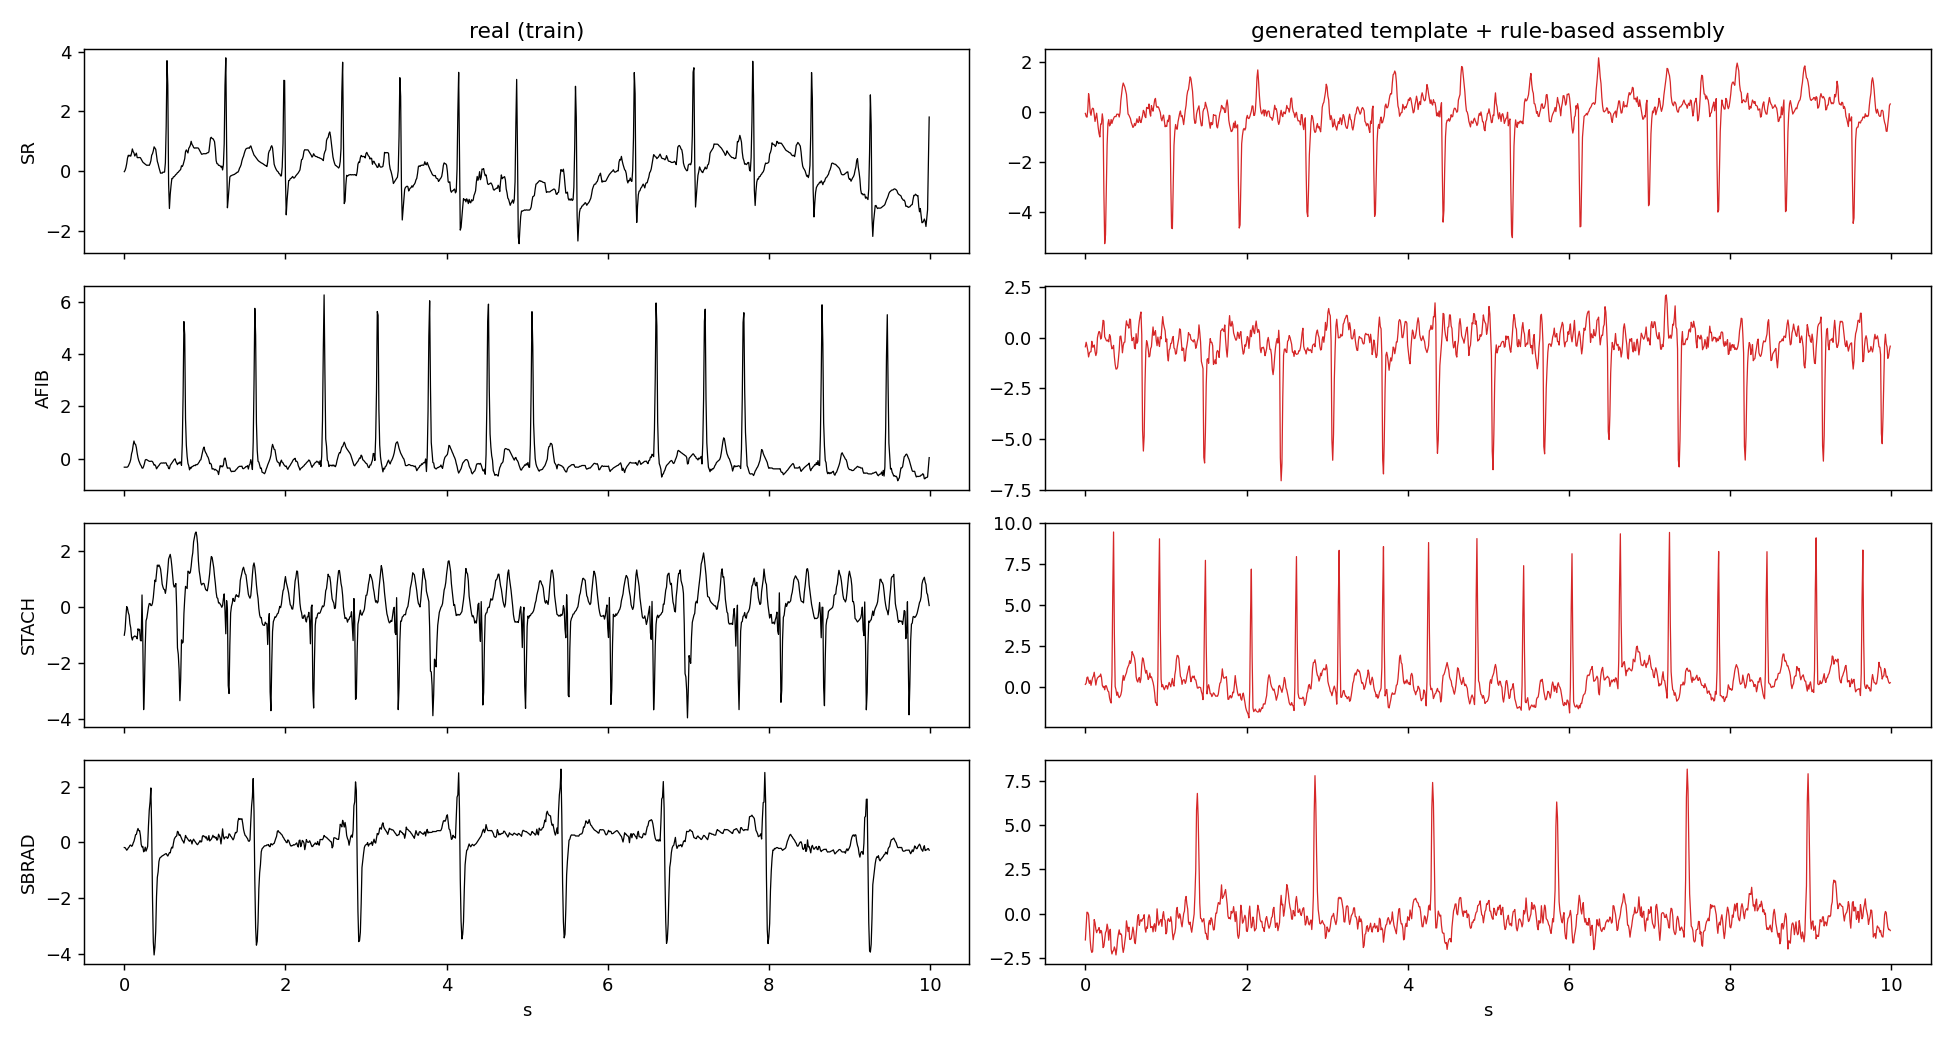
\includegraphics[width=0.78\linewidth]{fig2_ecgs.png}
\caption{Beat-stitched ECGs, one per class (lead II).}
\end{figure}

\begin{figure}[H]\centering
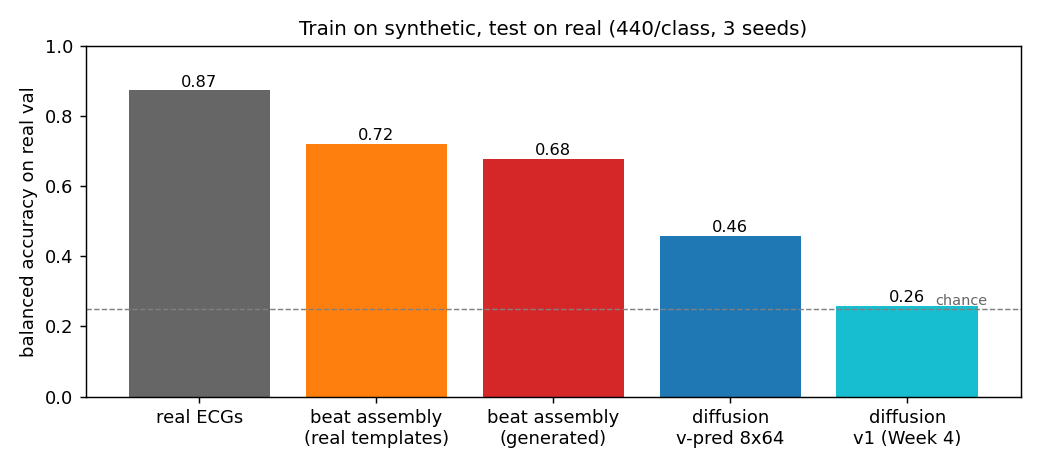
\includegraphics[width=0.8\linewidth]{fig3_tstr.png}
\caption{Train-on-synthetic, test-on-real balanced accuracy (440 ECGs per class, 3 seeds).}\label{fig:tstr}
\end{figure}

\obs
\begin{itemize}
\item Generated templates are as close to real templates as real templates are to each other: nearest-real
  correlation 0.89--0.93, against 0.88--0.94 real-to-real. None is a copy (none above 0.98).
\item Beat stitching keeps most of the class information: TSTR 0.678 with generated templates, 0.721 with real
  templates, 0.873 for real ECGs.
\item The early whole-ECG diffusion models (8$\times$64 and 16$\times$128 on raw signals) scored 0.26--0.46. They
  did not produce a regular heartbeat (Section~\ref{sec:fail}).
\end{itemize}

% ---------------------------------------------------------------- 4
\section{Quality Filtering and Augmentation}\label{sec:filter}
\subsection{The quality score}
\settings{Each synthetic ECG gets three within-class percentile ranks, which are averaged:
(1)~\emph{typicality}, meaning how typical its rhythm, per-lead amplitudes and spectral shape are for its class,
compared with real training ECGs;
(2)~\emph{realism}, the out-of-fold log-odds of a real-vs-synthetic detector;
(3)~\emph{label agreement}, the frozen baseline's probability of the intended class.
A variant without (3) checks that the filter does not simply pick ECGs the baseline already agrees with.}

\begin{table}[H]\centering\small
\begin{tabular}{lc}\toprule
synthetic ECGs used for training (440 per class) & balanced accuracy on real validation \\\midrule
top-scored & \textbf{0.743} \\
random & 0.672 \\
bottom-scored & 0.582 \\\bottomrule
\end{tabular}
\caption{Sanity check of the quality score (TSTR, pool of 3,200 AFIB / 1,800 STACH / 1,400 SBRAD).}
\end{table}

\subsection{Study 1 and Study 2: filtered vs random augmentation}
\settings{Each minority class is doubled with synthetic ECGs (+1,056 AFIB, +568 STACH, +446 SBRAD); SR is unchanged.
The conditions are: \emph{real} (nothing added), \emph{oversample} (real minority ECGs duplicated), \emph{random}
synthetic and \emph{filtered} synthetic (top-$k$ per class).
\emph{Study 2} (pre-registered): 4 independent synthetic pools $\times$ 10 seeds = 40 paired units per condition,
160 runs, a fixed budget of 6,250 steps, deterministic GPU training.}

\begin{figure}[H]\centering
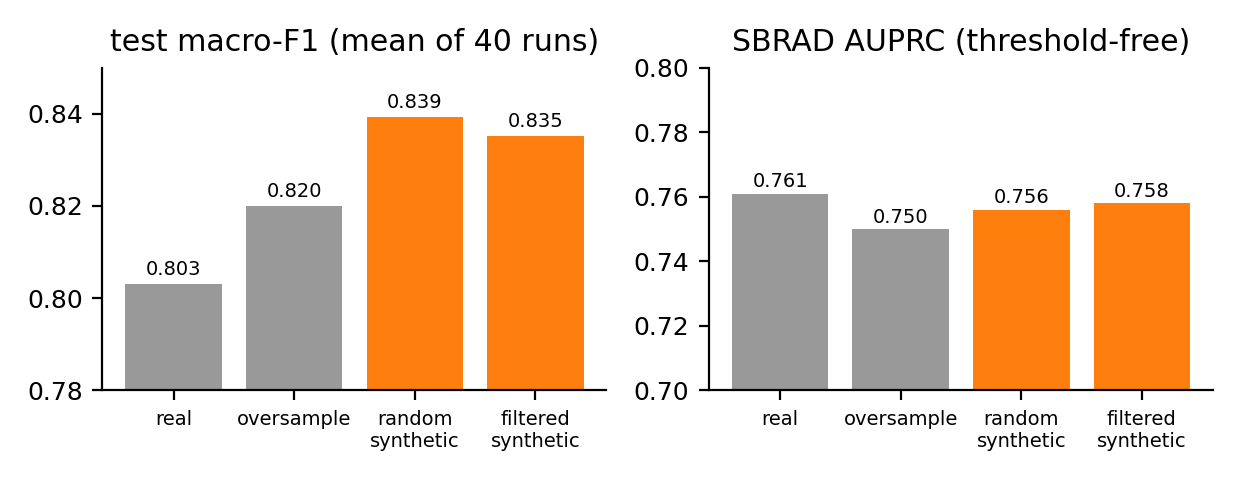
\includegraphics[width=0.78\linewidth]{fig_study2.png}
\caption{Study 2: test macro-F1 and SBRAD AUPRC by condition (mean of 40 runs).}\label{fig:study2}
\end{figure}

\begin{table}[H]\centering\small
\setlength{\tabcolsep}{4pt}\begin{tabular}{llccccp{3.0cm}}\toprule
 & comparison & mean diff. & wins & $p$ & 95\% CI & decision \\\midrule
H1 & filtered $-$ random & $-0.0041$ & 16/40 & 0.058 & $-0.012$ to $+0.003$ & not supported; equivalent within $\pm$0.01 \\
H2 & random $-$ real & $+0.0364$ & 40/40 & $<$0.0001 & $+0.026$ to $+0.047$ & supported \\
H3 & random $-$ oversample & $+0.0195$ & 37/40 & $<$0.0001 & $+0.008$ to $+0.031$ & supported \\\bottomrule
\end{tabular}
\caption[Study 2 registered hypotheses]{Study 2 registered hypotheses (test macro-F1; Holm-corrected; CI from a patient/seed/pool bootstrap).}
\end{table}

\obs
\begin{itemize}
\item \textbf{Filtering does not beat random selection.} Study 1 (10 + 30 seeds) found +0.0014 ($p=0.79$). A code
  review then found a selection bug: for STACH and SBRAD only 54\,\% and 38\,\% of the true top-$k$ were used. Study 2
  fixed it and found $-0.0041$, equivalent within $\pm$0.01.
\item \textbf{Why the score works alone but not as augmentation.} The score finds better \emph{standalone} samples
  (TSTR), but next to the full real training set that does not turn into a better classifier.
\item \textbf{Synthetic data beats real-only training and duplication}, but the gain is in precision: SBRAD F1 rises
  from 0.49 to 0.61 while SBRAD recall falls (0.81 $\rightarrow$ 0.77) and SBRAD AUPRC stays flat (0.761 vs 0.756).
  This points to a threshold effect (next section).
\end{itemize}

% ---------------------------------------------------------------- 5
\section{Scarcity and the Threshold Effect}\label{sec:threshold}
\subsection{Study 3: does synthetic data help more when real data is scarce?}
\settings{Each minority class is cut to 10, 25, 50 or 100\,\% of its patients (3 random draws). A fresh beat
generator is trained on each subset, so it never sees the dropped patients. The conditions are real, oversample and
synthetic, each with 5 seeds: 180 runs. Pre-registered; test macro-F1.}

\begin{table}[H]\centering\small
\begin{tabular}{lccc}\toprule
real minority kept & real & oversample & synthetic \\\midrule
10\,\% & 0.7588 $\pm$ 0.0176 & 0.7348 $\pm$ 0.0172 & \textbf{0.7615} $\pm$ 0.0162 \\
25\,\% & 0.7986 $\pm$ 0.0146 & 0.8228 $\pm$ 0.0112 & \textbf{0.8347} $\pm$ 0.0117 \\
50\,\% & 0.8047 $\pm$ 0.0127 & 0.8348 $\pm$ 0.0129 & \textbf{0.8530} $\pm$ 0.0138 \\
100\,\% & 0.7960 $\pm$ 0.0090 & 0.8201 $\pm$ 0.0104 & \textbf{0.8399} $\pm$ 0.0110 \\\bottomrule
\end{tabular}
\caption{Study 3: test macro-F1 (mean $\pm$ SD over 15 units).}
\end{table}

\begin{figure}[H]\centering
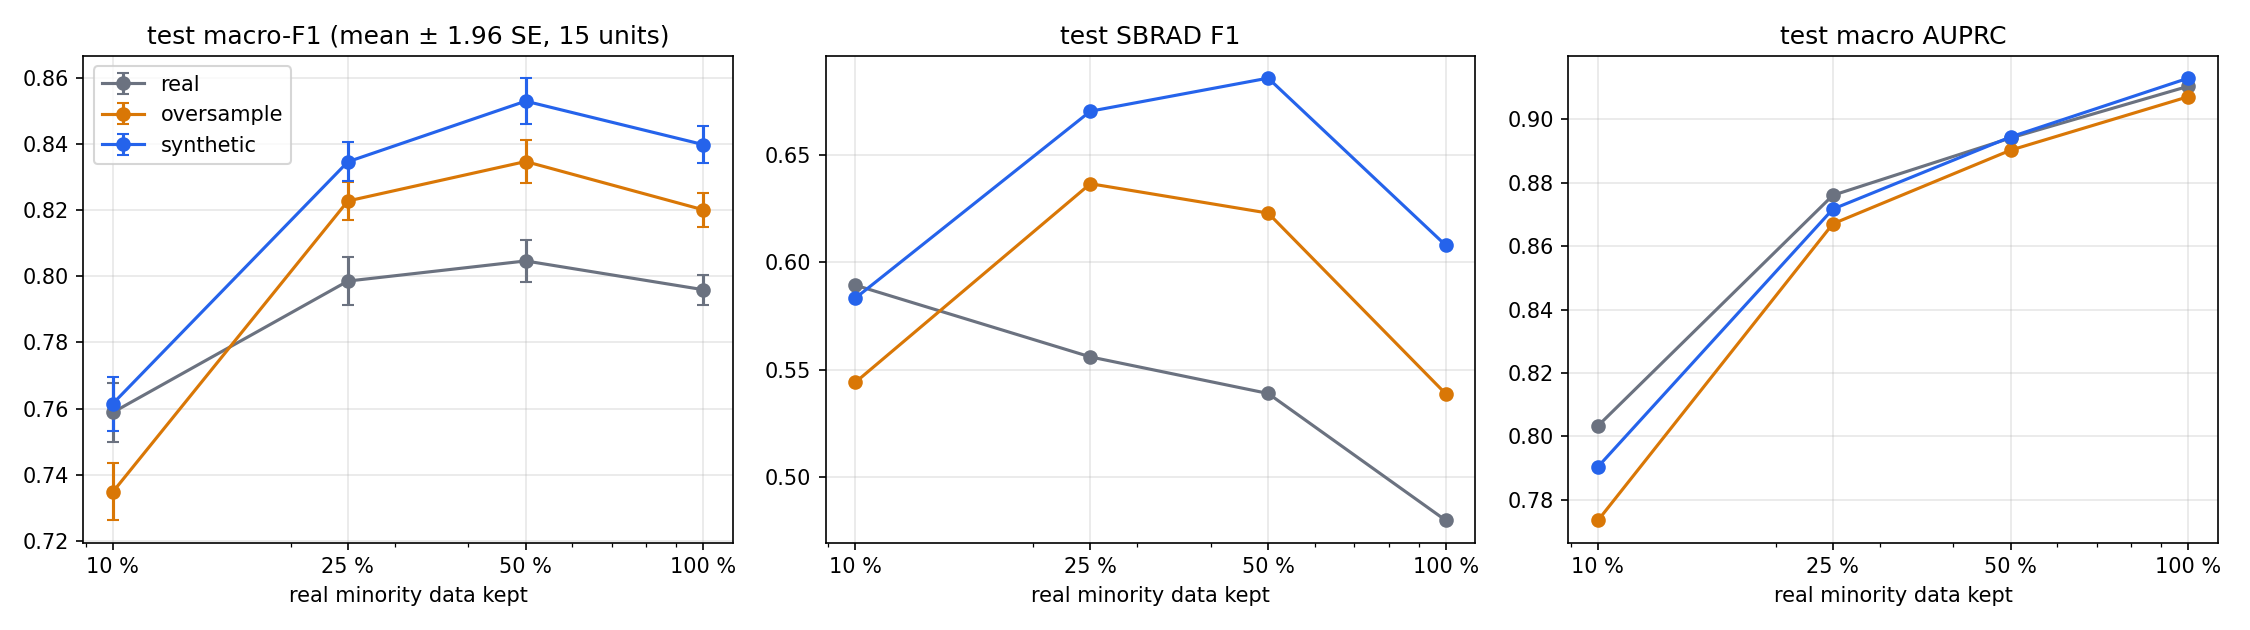
\includegraphics[width=0.95\linewidth]{fig_study3_curves.png}
\caption{Study 3: macro-F1, SBRAD F1 and macro AUPRC by amount of real minority data.}
\end{figure}

\obs
\begin{itemize}
\item \textbf{No extra benefit at 10\,\%} (primary H1: +0.0027, $p=0.60$, not supported). The gain over real-only
  appears at 25--100\,\% (+0.04 to +0.05).
\item Synthetic beats oversampling at every level, robustly only at 50 and 100\,\%. The gain does not grow as data
  shrinks (H3, H4 not supported).
\item Macro AUPRC is about the same for all conditions, as in Study 2.
\end{itemize}

\subsection{Is the gain a threshold effect?}
\settings{All 180 Study 3 classifiers are reused without retraining. Per-class log-probability offsets
($b_{\mathrm{SR}}=0$) are tuned to maximise macro-F1 on one half of the validation patients and scored on the other
half. This analysis was exploratory and not pre-registered.}

\begin{figure}[H]\centering
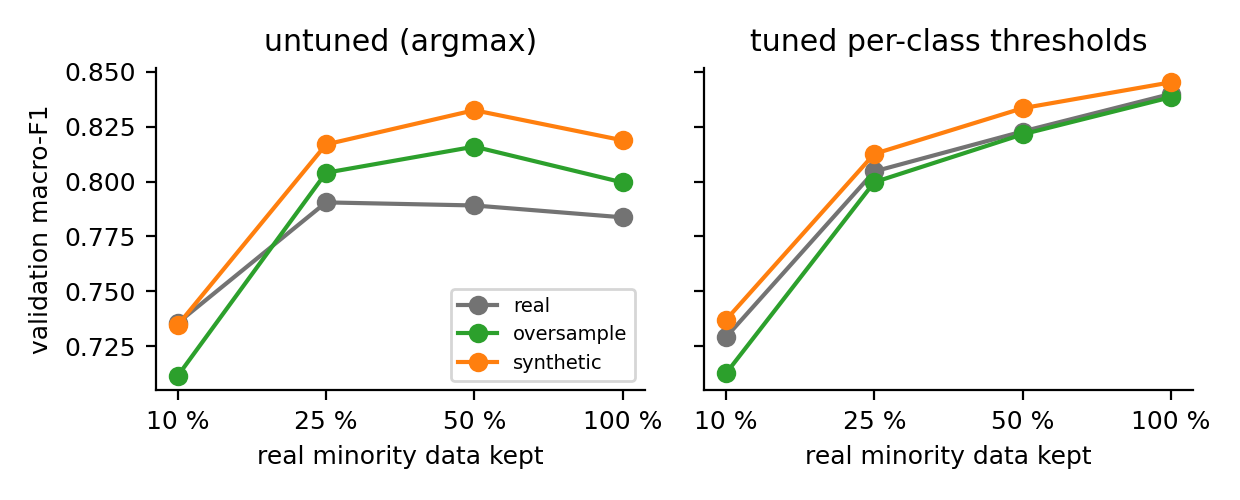
\includegraphics[width=0.9\linewidth]{fig_threshold.png}
\caption{Validation macro-F1 before and after per-class threshold tuning (15 runs per point).}\label{fig:threshold}
\end{figure}

\obs
\begin{itemize}
\item \textbf{Tuning closes most of the gap:} 69.9\,\%, 76\,\% and 85\,\% of the synthetic $-$ real gap at 25, 50 and
  100\,\%. What remains is +0.005 to +0.011 macro-F1.
\item The real-only model over-predicts SBRAD (precision 0.33--0.43). A negative SBRAD offset fixes most of that. At
  100\,\%, a tuned real-only model beats the untuned synthetic one.
\item The same pattern appears in Study 4 (Section~\ref{sec:realism}) and in the latent diffusion utility test
  (Section~\ref{sec:scale}): synthetic augmentation acts mainly as decision-threshold calibration.
\end{itemize}

% ---------------------------------------------------------------- 6
\section{Why Synthetic ECGs Are Detectable}\label{sec:realism}
\settings{Study 4 used only the training and validation splits. A gradient-boosted judge on 25 standard ECG features
is trained to separate real from beat-stitched ECGs, with patient-grouped splits. Controls: real vs real and real vs
real-rebuilt (each real ECG reassembled from its own template and residual).}

\begin{table}[H]\centering\small
\begin{tabular}{lcc}\toprule
feature & real & beat stitching \\\midrule
residual (non-template) kurtosis & 30 & 9 \\
beat-to-template correlation & 0.96 & 0.82 \\
noise and baseline-wander level & 1$\times$ & 1.65--1.7$\times$ \\
R-peak detector errors (own detector) & 0\,\% & 11\,\% missed, 20\,\% spurious \\
QRS width, R/S/T amplitude, ST level & \multicolumn{2}{c}{not separable (feature AUC 0.44--0.55)} \\\bottomrule
\end{tabular}
\caption{What gives beat-stitched ECGs away (judge AUC 0.973; controls 0.509 and 0.512).}
\end{table}

\obs
\begin{itemize}
\item \textbf{Beats are realistic; the assembly is not.} The giveaways are the hand-built noise and the beat-to-beat
  variation. The noise model also makes 30--51\,\% of regular-rhythm ECGs look as irregular as AFIB to R-peak
  detectors.
\item \textbf{Fixing the noise did not reach realism.} A learned residual model (conditional diffusion) cut
  beat-detection errors 3$\times$ but stayed fully detectable (Section~\ref{sec:fail}).
\item \textbf{Usefulness does not depend on the noise.} Synthetic pools that differ only in noise (none, learned,
  hand-built) all give +0.025 to +0.029 untuned macro-F1, about 0 AUPRC and about 0 tuned macro-F1 (10 seeds,
  validation). This is a third replication of the threshold effect.
\end{itemize}

% ---------------------------------------------------------------- 7
\section{Generator 2: Latent Diffusion}\label{sec:latent}
\settings{Instead of stitching beats, a single model generates the whole 10-second ECG.
\emph{Autoencoder}: compresses 12$\times$1000 to a 16$\times$125 latent. It is retrained for 60 epochs (rung r1),
because the original version smoothed baseline wander.
\emph{Diffusion model}: an SSSD-style S4 denoiser in the latent space with a cosine schedule (1000 steps),
v-prediction, classifier-free guidance on class and heart rate, an EMA of 0.999, class-balanced and HR-stratified
sampling, and AdamW $2\times10^{-4}$.
\emph{Model C}: 8 layers $\times$ 64 (0.8\,M parameters).
\emph{Model D}: as C, plus an R-peak map (Gaussian bumps at the requested beat positions) for rhythm control.
Both were trained on fit patients, and every choice was made on dev.}

\subsection{Evaluation protocol}
Realism is measured with the feature judge against two reference levels. The \textbf{floor} (real vs real, 0.454 on
validation) shows what "indistinguishable" looks like at this sample size. The \textbf{ceiling} (real vs autoencoder
reconstruction) is the best any model decoding through this autoencoder can reach. Diversity is measured by
task-embedding coverage, heart rate by HR-W, and copying by a membership test. All intervals resample patients.

\begin{table}[H]\centering\small
\begin{tabular}{lccc}\toprule
autoencoder & judge AUC (dev) & noise/wander group & passes ceiling gate ($\le$ 0.65)? \\\midrule
original (v1) & 0.718 $\pm$ 0.025 & 0.724 & no \\
retrained, 60 epochs (r1) & \textbf{0.625} $\pm$ 0.025 & 0.621 & yes (validation: 0.627) \\\bottomrule
\end{tabular}
\caption{Autoencoder reconstruction ceiling.}
\end{table}

\subsection{Results on dev}
\begin{table}[H]\centering\small
\begin{tabular}{lccccc}\toprule
dev pool (571 ECGs) & full judge & rhythm judge & HR-W (bpm) & coverage & rhythm failures \\\midrule
beat stitching (hybrid) & 0.970 & 0.720 & 6.81 & 0.758 & 4.1\,\% \\
latent diffusion v1 & 1.000 & 0.982 & 23.3 & 0.518 & 61.7\,\% \\
C, 60k steps & 0.967 & 0.841 & 6.22 & 0.962 & 11.9\,\% \\
C, 120k steps & \textbf{0.922} & 0.743 & 3.55 & 0.971 & 3.1\,\% \\
D, 60k steps & 0.983 & 0.624 & 4.33 & 0.872 & 4.7\,\% \\
D, 120k steps & 0.967 & \textbf{0.570} & 3.65 & 0.869 & 1.9\,\% \\\bottomrule
\end{tabular}
\caption{Latent diffusion on dev (classifier-free guidance 2, 50 DDIM steps; sampler chosen on dev).}
\end{table}

\begin{figure}[H]\centering
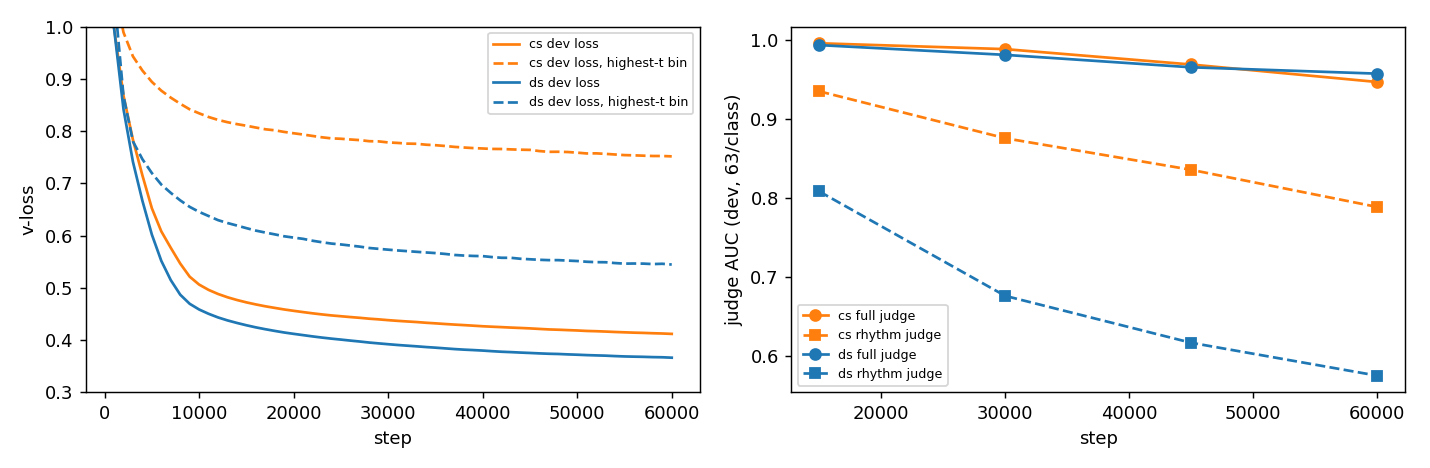
\includegraphics[width=0.9\linewidth]{training_curves.png}
\caption{Dev loss and dev judge AUC during training of C and D (first 60k steps).}
\end{figure}

\begin{figure}[H]\centering
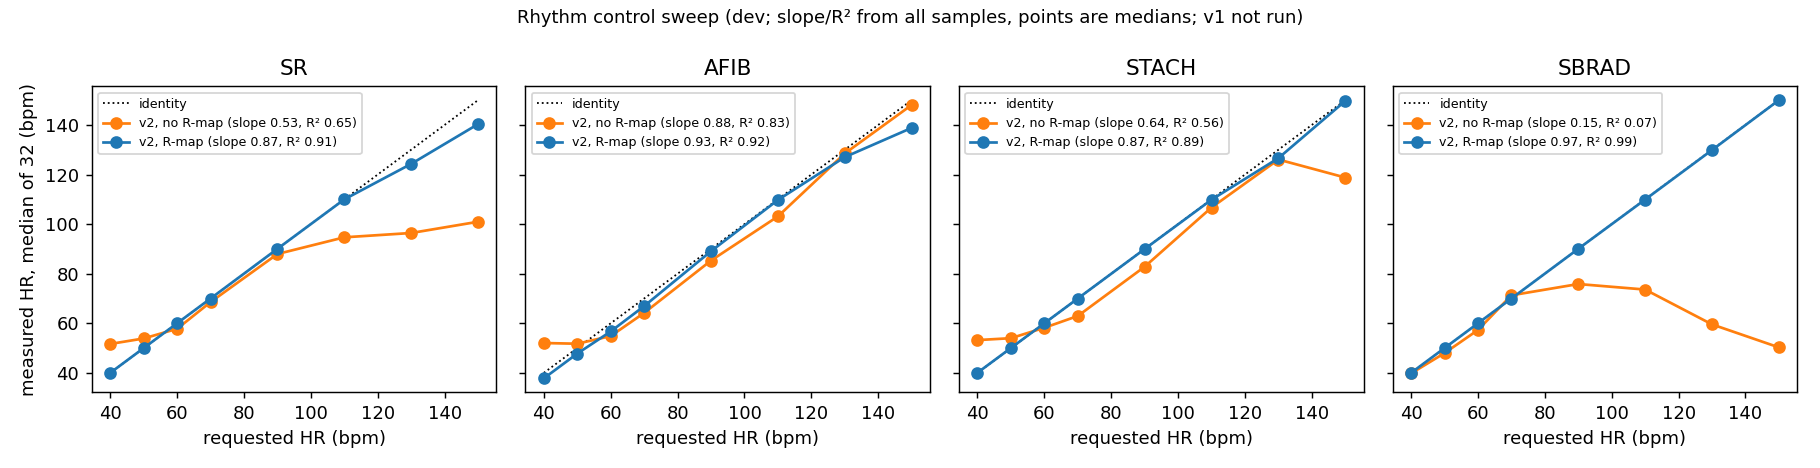
\includegraphics[width=\linewidth]{rhythm_sweep.png}
\caption{Requested vs measured heart rate for C (no R-peak map) and D (R-peak map), 60k steps.}\label{fig:sweep}
\end{figure}

\obs
\begin{itemize}
\item \textbf{Training length matters.} From 60k to 120k steps, C's dev judge falls from 0.967 to 0.922, although its
  dev loss changes little (0.412 $\rightarrow$ 0.394). Checkpoints are therefore chosen by realism, not by loss.
\item \textbf{Rhythm conditioning works in the medians, not by the registered gate.} D follows the requested heart
  rate almost exactly from 40 to 110\,bpm. The pre-registered slope rule (0.9--1.1 in SR, STACH and SBRAD) still
  failed, partly because the sweep asked for sinus rhythm at 130--150\,bpm, which clinically is tachycardia. D also has the best
  rhythm judge, but worse waveform realism: QRS amplitude is about 1.5$\times$ too large at guidance 2, and 0.8--0.9$\times$ at
  guidance 1.
\item \textbf{Model C has the most variety} (coverage 0.96--0.97, against 0.76 for beat stitching).
\end{itemize}

% ---------------------------------------------------------------- 8
\section{Scaling Up on Colab and Kaggle}\label{sec:scale}
\settings{\textbf{C-M}: the same model as C with 16 layers $\times$ 128 width and S4 state 64 (5.87\,M parameters),
on the same latents, sampler, learning rate and seed. Training ran on a Google Colab T4 for steps 0--54k and on a Kaggle GPU for steps 54k--100k, resuming from the
checkpoint with its optimizer and random-number states.}

\subsection{An S4 kernel mismatch between machines}
The S4 layer computes a Cauchy kernel by one of three code paths. The fast paths (pykeops, or a CUDA extension) sum
over conjugate pairs of state values. The fallback, used on the laptop, sums only the stored half. Weights trained on
one path therefore give a different network on the other. When the dev loss of C-M (trained with pykeops) was
recomputed on the laptop, it gave 0.662 instead of the logged 0.4193. With the fallback patched in memory to sum
conjugate pairs, it matched exactly (0.4193). The laptop models (C, D) match their logged loss on the fallback path.
All C-M results here use the matching kernel (\texttt{latent\_diffusion/s4\_kernel.py}). The first C-M scores, made on
the wrong path, were discarded.

\begin{figure}[H]\centering
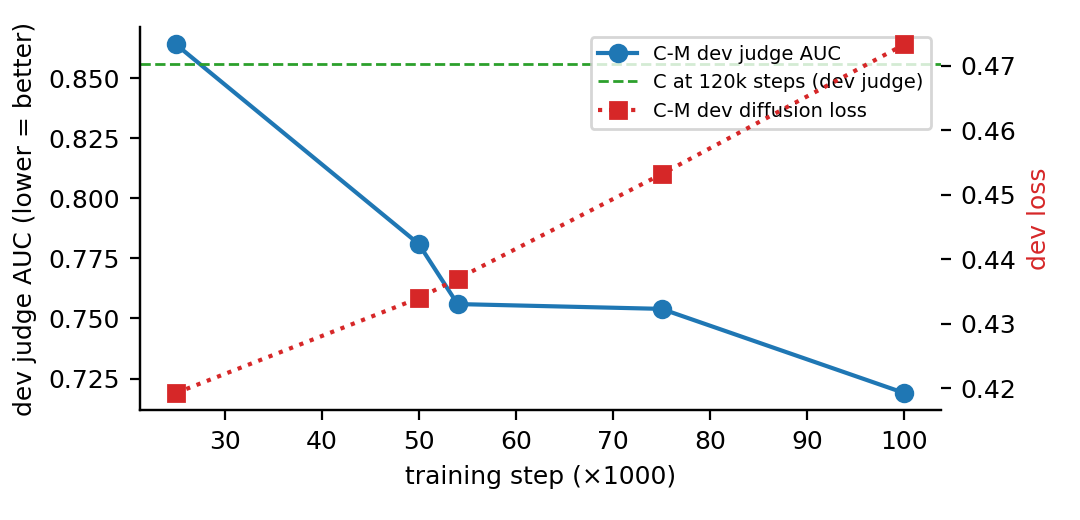
\includegraphics[width=0.62\linewidth]{fig_cm_checkpoints.png}
\caption{C-M checkpoints on dev: judge AUC keeps improving while dev loss rises.}\label{fig:cm}
\end{figure}

\subsection{Validation result (pre-registered second look)}
\settings{Same validation patients (256 SR / 224 AFIB / 125 STACH / 96 SBRAD), floor, reference and decision rule as
the original validation benchmark. A pool is \emph{better} than the hybrid if its judge mean $+$ 2 SD lies below the
hybrid's mean $-$ 2 SD \emph{and} coverage and HR-W are not worse in at least 3 of 4 classes. Checkpoints were
selected on dev (C-M: best of 25k/50k/54k/75k/100k).}

\begin{figure}[H]\centering
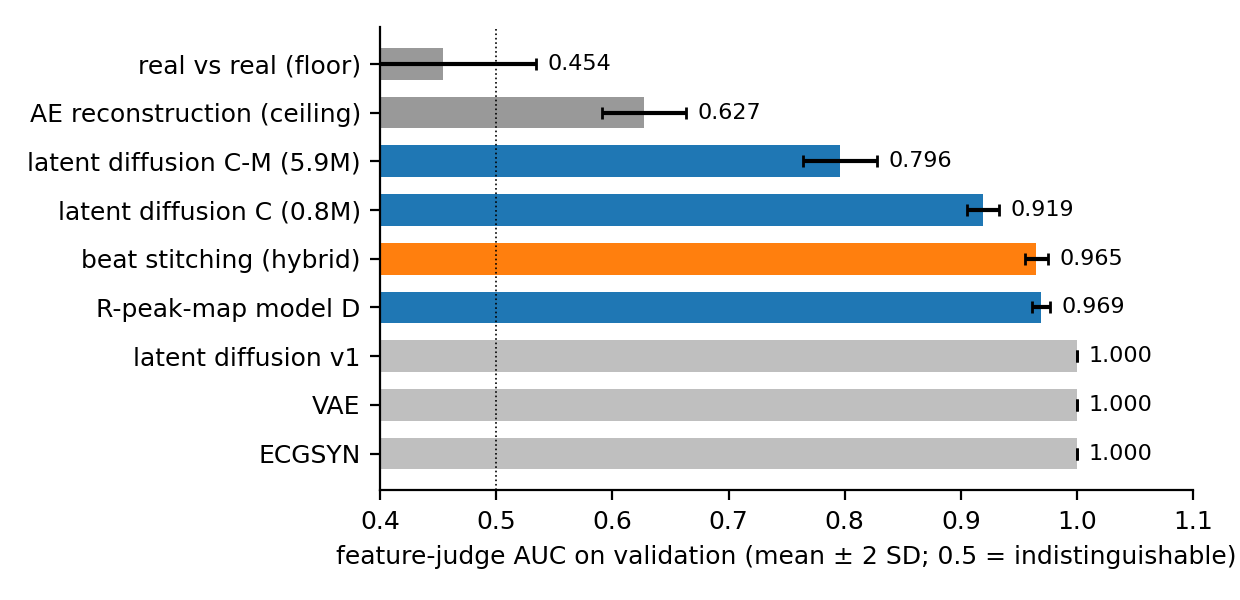
\includegraphics[width=0.72\linewidth]{fig_realism_ladder.png}
\caption{Realism on validation for all generators, with floor and ceiling.}\label{fig:ladder}
\end{figure}

\begin{table}[H]\centering\small
\setlength{\tabcolsep}{4pt}\begin{tabular}{lcccccccc}\toprule
pool & full & rhythm & morph. & noise & global & HR-W & cov. & verdict \\\midrule
real vs real (floor) & 0.454 & 0.495 & 0.522 & 0.448 & 0.484 & 2.70 & 0.952 & -- \\
beat stitching (hybrid) & 0.965 & 0.735 & 0.882 & 0.959 & 0.766 & 8.35 & 0.750 & reference \\
C, 120k & 0.919 & 0.727 & 0.818 & 0.845 & 0.723 & 2.61 & 0.962 & better \\
D, 120k (R-peak map) & 0.969 & 0.592 & 0.954 & 0.896 & 0.907 & 2.60 & 0.816 & not disting. \\
\textbf{C-M, 100k} & \textbf{0.796} & 0.626 & \textbf{0.723} & \textbf{0.729} & \textbf{0.613} & \textbf{2.29} & 0.957 & \textbf{better} \\\bottomrule
\end{tabular}
\caption{Validation feature judges (full and per feature group), HR-W and coverage. C-M SD 0.016; sampling-run spread 0.795--0.818.}
\end{table}

\begin{figure}[H]\centering
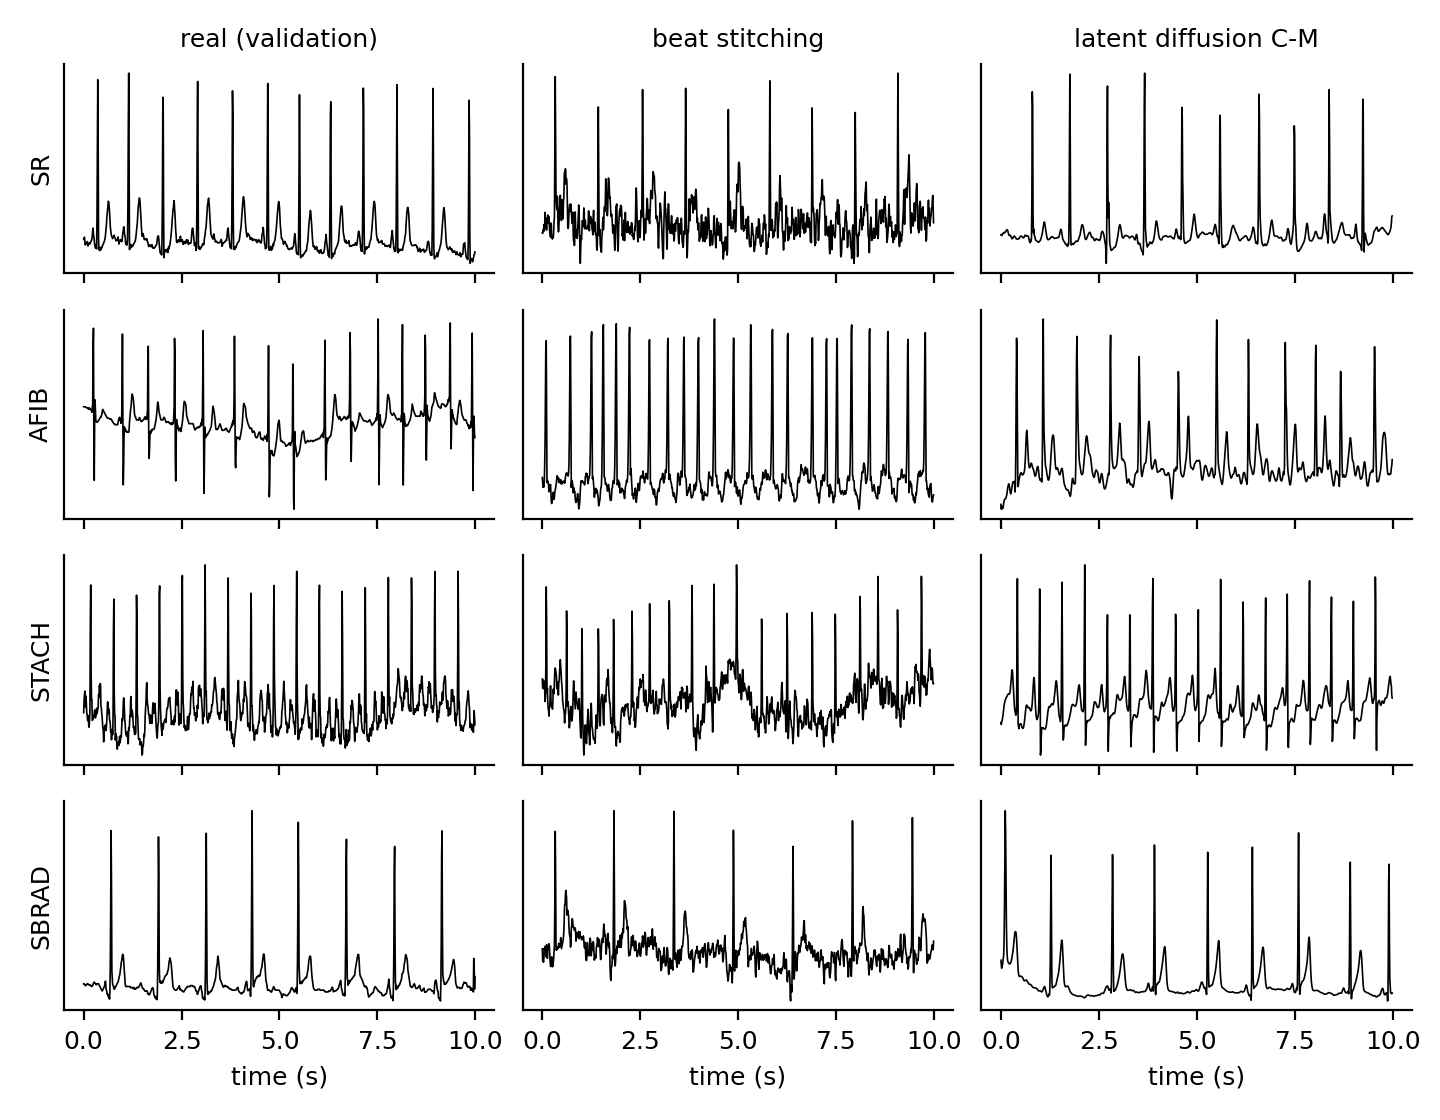
\includegraphics[width=0.8\linewidth]{fig_examples.png}
\caption{Lead II, one random ECG per class: real validation, beat stitching and C-M.}\label{fig:examples}
\end{figure}

\obs
\begin{itemize}
\item \textbf{C-M is the most realistic generator}, and better than beat stitching by the pre-registered rule. It
  improves in every feature group: morphology, noise/wander, rhythm and global features. Its sampling runs
  (0.795--0.818) all stay far below the hybrid.
\item \textbf{The rising dev loss was not overfitting of the samples.} Dev loss rose from 0.419 to 0.473 while dev
  realism improved from 0.864 to 0.719 (Figure~\ref{fig:cm}).
\item \textbf{No copying.} There are no exact copies, and membership AUC is 0.48--0.56 in every class.
\item \textbf{Still clearly synthetic.} The gap to the floor (0.454) and to the autoencoder ceiling (0.627) shows room
  for improvement.
\item \textbf{Utility repeats the threshold effect.} With the same 6,250-step recipe on validation (5 seeds),
  latent-diffusion augmentation (model C) raises untuned macro-F1 (0.786 $\rightarrow$ 0.803), like beat stitching
  (0.817) and oversampling (0.809). AUPRC (0.883 real, 0.877 latent) and tuned macro-F1 (0.845 real, 0.832 latent)
  do not improve. The augmentation value of C-M itself was not measured.
\end{itemize}

% ---------------------------------------------------------------- 9
\section{What Did Not Work}\label{sec:fail}
\begin{table}[H]\centering\small
\begin{tabular}{p{5.0cm}p{9.6cm}}\toprule
attempt & outcome \\\midrule
Whole-ECG SSSD on raw signals, 8$\times$64 and 16$\times$128 & No regular heartbeat (periodicity 0.13--0.25 vs 0.84 real); TSTR 0.26--0.46. $\varepsilon$-prediction could not even memorise one ECG; v-prediction could, but plateaued. \\
Noise-schedule, EMA, class-balancing, 80$\times$ budget & Fixed amplitude and spectrum, not rhythm. \\
Envelope-modulated noise; template-relative beat variation & Judge 0.998 and 0.94: no closer to real. \\
Real beat variation borrowed from other patients & 0.83: better than modelled variation, but did not meet the realism bar. \\
Learned residual (conditional diffusion) & Detector still 1.000; kurtosis 4--9 vs 23--39 real; 3$\times$ fewer R-peak errors. \\
Latent diffusion v1, VAE, ECGSYN baselines & All judge 1.000; HR-W 19--28\,bpm. \\
R-peak-map conditioning (model D) & Better rhythm, worse morphology; failed its registered gate. \\\bottomrule
\end{tabular}
\caption{Approaches that did not reach their goal, and what each one showed.}
\end{table}

% ---------------------------------------------------------------- 10
\section{Limitations}
\begin{itemize}
\item \textbf{Test-split reuse.} Studies 1--3 used the same test split for several registered analyses. The latent
  diffusion results use validation, which was looked at twice (the original benchmark and the pre-registered second
  look). Checkpoints were selected on dev.
\item \textbf{C-M was evaluated for realism only}, not for augmentation utility.
\item \textbf{One training seed per generator}, one dataset (PTB-XL), one classifier architecture.
\item \textbf{The judge is one realism measure.} It uses 25 clinical features at about 100--250 ECGs per class.
  Values near 1 are compressed, and no clinician reader study was done.
\item \textbf{Heart rate and R-peaks come from a heuristic detector}, both for conditioning and for evaluation.
\item \textbf{No published generator was scored} with this protocol (for example SSSD-ECG), so no claim is made
  against the state of the art.
\item \textbf{Hardware.} A 4\,GB laptop GPU limited the model size; the largest model needed cloud GPUs and the
  matching S4 kernel.
\end{itemize}

\clearpage
% ---------------------------------------------------------------- 11
\section{Summary of Main Insights}
\begin{itemize}
\item \textbf{A learned beat model plus a hand-built rhythm is a strong first generator}, but its hand-built noise is
  what gives it away. Beat morphology itself is realistic.
\item \textbf{Sample quality on its own is not augmentation value.} The quality score finds better standalone
  samples, yet filtered and random synthetic data help a classifier equally.
\item \textbf{Synthetic augmentation mainly recalibrates decision thresholds.} The untuned F1 gains replicate across
  studies, generators and noise models. A tuned real-only classifier recovers most of them, and AUPRC does not move.
\item \textbf{Scale and training time make latent diffusion work.} A 5.9\,M-parameter latent model trained for 100k
  steps is clearly more realistic than beat stitching on held-out validation patients (0.796 vs 0.965), with more
  variety and without copying.
\item \textbf{Evaluate generators against a floor and a ceiling, and choose checkpoints by realism.} The diffusion
  loss stopped tracking sample quality late in training.
\end{itemize}

% ---------------------------------------------------------------- appendix
\clearpage
\appendix
\section{Reproducibility}
\begin{table}[H]\centering\small
\begin{tabular}{p{3.3cm}p{11.3cm}}\toprule
step & command (from the repository root) \\\midrule
data & PTB-XL 1.0.1 into \path{archive/}; run \path{notebooks/02_PTBXL_Exploration.ipynb} \\
beat stitching & \path{py -m studies.beat_generator._run_template_gen}, then \path{studies.beat_generator._beat_gen_pool} (checkpoint \path{generator_comparison/template_gen/checkpoints/tpl_8x64_last.pt}) \\
quality score & \path{py -m generator_comparison.quality_filter <pool> <out>} \\
Studies 1--4 & \path{studies/study1/} \dots\ \path{studies/study4/}, e.g.\ \path{py -m studies.study2._run_study2}, then \path{studies.study2._study2_analysis}; threshold tuning: \path{studies.study3._threshold_explore} (see \path{studies/README.md}) \\
latent diffusion (C, D) & \path{py -m latent_diffusion.train_diffusion_v2 --name cs --steps 120000} (add \path{--rhythm} for D) \\
C-M & \path{latent_diffusion/colab/ECG_colab_CM.ipynb} and \path{ECG_kaggle_CM.ipynb} (16$\times$128, state 64, 100k steps) \\
evaluation & \path{latent_diffusion/dev_eval_v2.py}, \path{eval_120k_v2.py}, \path{phase_f_v2.py}, \path{phase_f2_second_look.py} \\
figures & \path{report/make_figures.py} \\\bottomrule
\end{tabular}
\caption{Commands and files.}
\end{table}

\noindent\textbf{Checkpoints in the repository.} C-M (\path{diffusion_cm/step100000.pt}, EMA weights only, 31\,MB;
sample inside \path{conj_kernel()}), C and D (\path{diffusion_cs/last.pt}, \path{diffusion_ds/last.pt}),
the autoencoder (\path{ae_r1/best.pt}), the beat-template generator and the CNN-LSTM baseline.
\textbf{Seeds:} split 42; latent diffusion training 9200; validation sampling 9620 (extra runs 9630--9632).
\textbf{Hardware:} RTX 3050 Laptop 4\,GB (Python 3.14, PyTorch 2.11), Colab T4 and Kaggle GPU.
\textbf{Pre-registrations:} \path{report/PREREGISTRATION.md}, \path{_2}, \path{_3}, and
\path{latent_diffusion/audits/v2/amendment1.md} (amendments 1--8).

\end{document}
